\begin{figure}[t]
  \centering
  \begin{subfigure}[b]{0.39\textwidth}
    \centering
  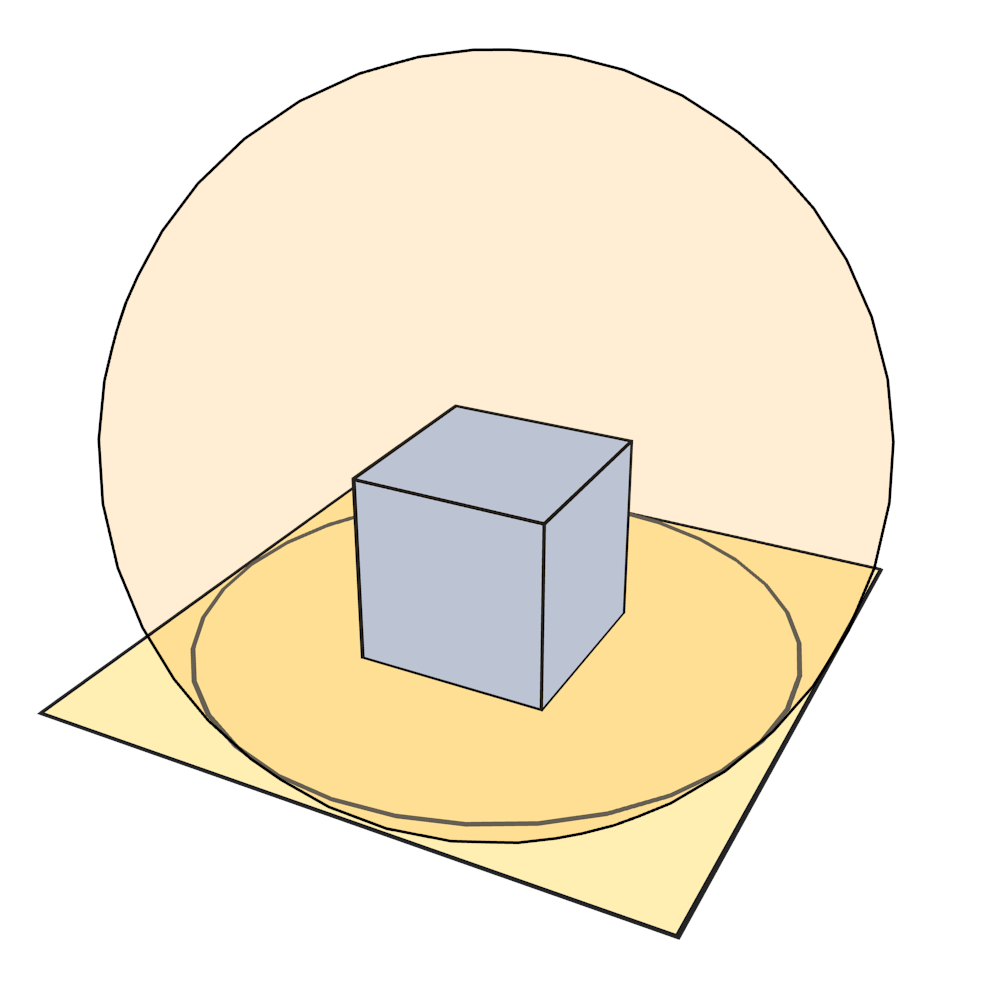
\includegraphics[width=\textwidth]{./img/raw/besluit-geom/scene.png}
  \caption{Simpele sc\'ene.}
  \label{fig:vo-geometrie:0}
  \end{subfigure}%
  \begin{subfigure}[b]{0.39\textwidth}
    \centering
  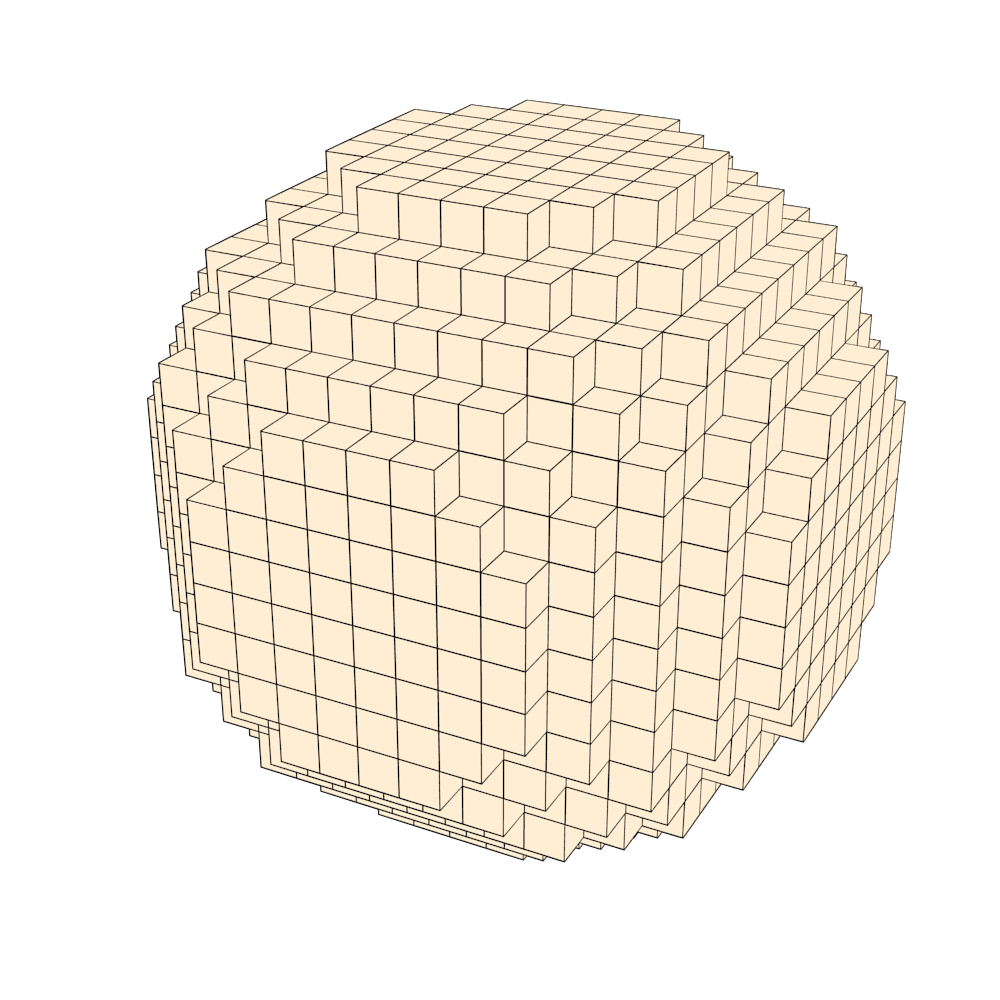
\includegraphics[width=\textwidth]{./img/raw/besluit-geom/light.png}
  \caption{Lichtknopen.}
  \label{fig:vo-subsets:1}
  \end{subfigure}\\
  \begin{subfigure}[b]{0.39\textwidth}
    \centering
  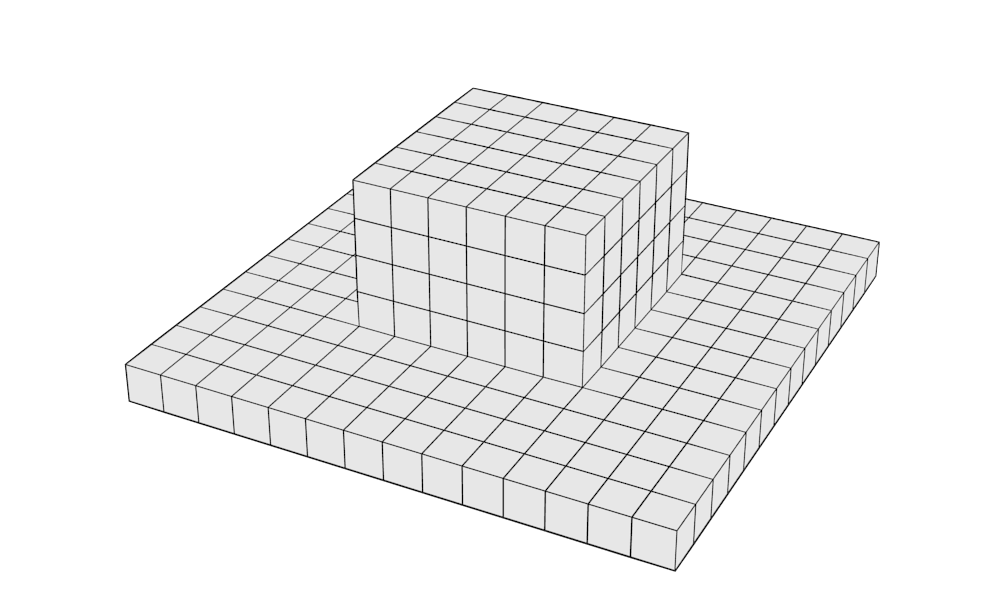
\includegraphics[width=\textwidth]{./img/raw/besluit-geom/geom.png}
  \caption{Geometrieknopen.}
  \label{fig:vo-geometrie:0}
  \end{subfigure}%
  \begin{subfigure}[b]{0.39\textwidth}
    \centering
  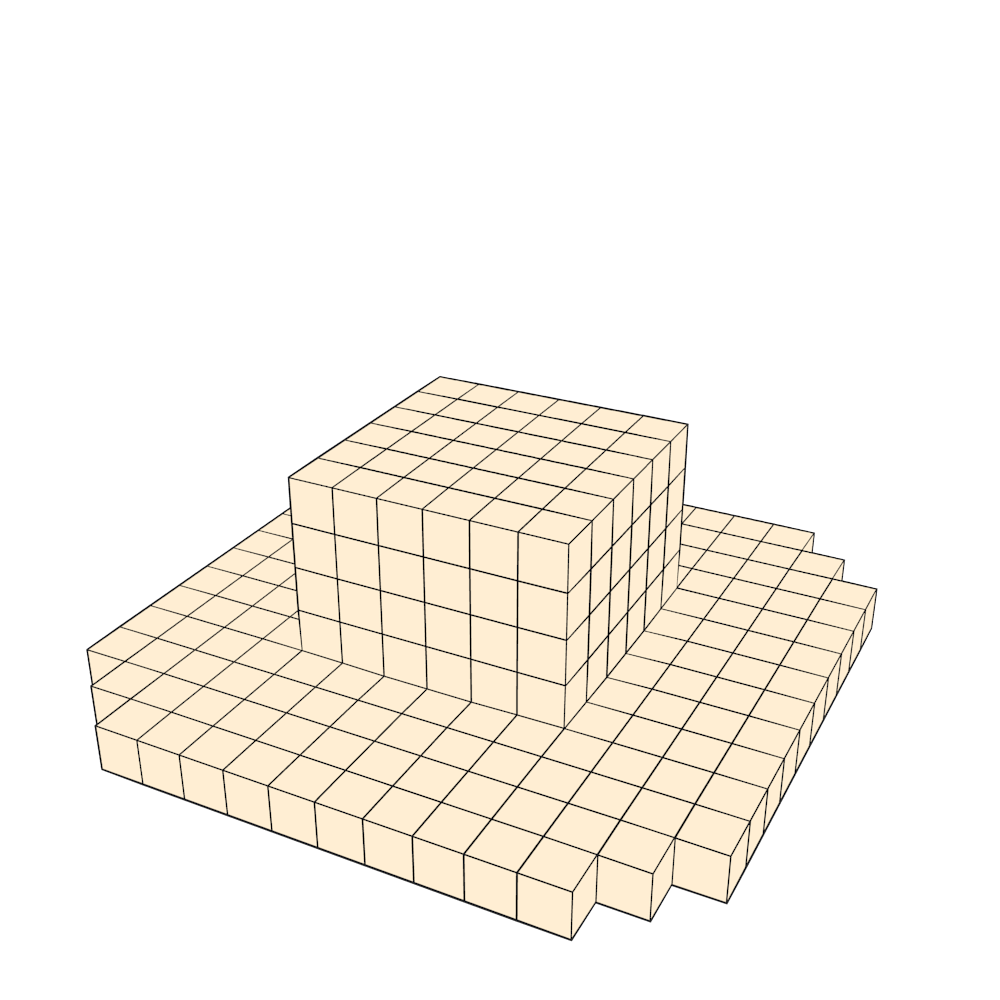
\includegraphics[width=\textwidth]{./img/raw/besluit-geom/comb.png}
  \caption{Licht-geometrie-knopen.}
  \label{fig:vo-subsets:1}
  \end{subfigure}
  \caption{Reductie van het aantal lichtknopen met behulp van de geometrie.}
  \label{fig:vo-geometrie}
\end{figure}
